\section{Introduction}
The proliferation of learning-based applications such as recommender systems, fraud detection, and automated content tagging, has encouraged the development of advanced statistical analytics libraries integrated with the data management stack \cite{bdas, alexandrov2014stratosphere, crotty2014tupleware, hellerstein2012madlib}. 
While these libraries significantly reduce the required effort in developing scalable learning applications, acquiring ``clean" data of sufficient quality for learning is still a bottleneck.
Data are susceptible to various forms of corruption such as missing, incorrect, or inconsistent representations, and industrial surveys have established that dirty data are prevalent  \cite{Gartner}.
Data corruption, when systematic \cite{taylor1982introduction} (i.e., correlated with the data), can bias learning algorithms and lead to error-prone predictions \cite{xiaofeature}.

An important class of these new advanced analytics, supervised machine learning, relies on correlating features with labels.
Systematically corrupted data can lead to confouding correlations between features and labels.
Consider a music recommender system in which due to a software bug, all users from Europe have an incorrect age attribute defaulted to ``18-24".
A recommendation model trained on this data may spuriously ``learn" a correlation relationship between the ``18-24" age group and music liked by European users.
While there is an extensive literature on robust Machine Learning, this work largely focuses on resilience to atypical outliers (i.e., age ``150") and not spurious correlations.

Such problems can be ameliorated by a variety of data cleaning techniques (see Rahm and Do \cite{rahm2000data} for a survey).
Recently, several scalable data cleaning frameworks have been proposed including BigDansing\cite{khayyat2015bigdansing}, SampleClean\cite{sampleclean}, and Katara \cite{chu2015katara}. 
Unfortunately, even with recently researched optimizations, data cleaning can be time consuming and economically infeasible\cite{wang1999sample}.
Programming data transformations to fix all problems manifest in the data requires substantial developer effort \cite{kandel2012}.
When scripted transformations do not suffice, crowdsourcing is a popular alternative with recent success in missing value filling and entity resolution \cite{gokhale2014corleone, park2014crowdfill, sampleclean,chu2015katara}.
However, crowdsourcing comes at the cost of additional latency, overhead of managing human workers, and significant monetary expense.

Thus, for many corrupted datasets, the analyst can only practically clean $k \ll N$ records.
However, budgeted data cleaning poses a few problematic methodological issues when applied before model training.
First, mixing dirty and clean data violates homogeneity assumptions and can lead to dramtically incorrect models in even simple scenarios (Figure \ref{update-arch1}).
To avoid this problem, we could use a random sampling approach (e.g., \cite{wang1999sample}), where the analyst first samples $k$ records, applies data cleaning to this subset, and then trains a model using only the clean data.
While this avoids the earlier problem, model training can require a large amount of training data and $k$ examples may not be enough to support viable predictions.
Furthermore, if errors are sparse, any random sampling-based approach will largely select already cleaned data leading to wasted effort.
Under strict cleaning budgets, the errors introduced by sampling or mixing may dominate any gains from data cleaning, leading to unreliable or even misleading conclusions about data or model quality.

\begin{figure}[t]
\centering
 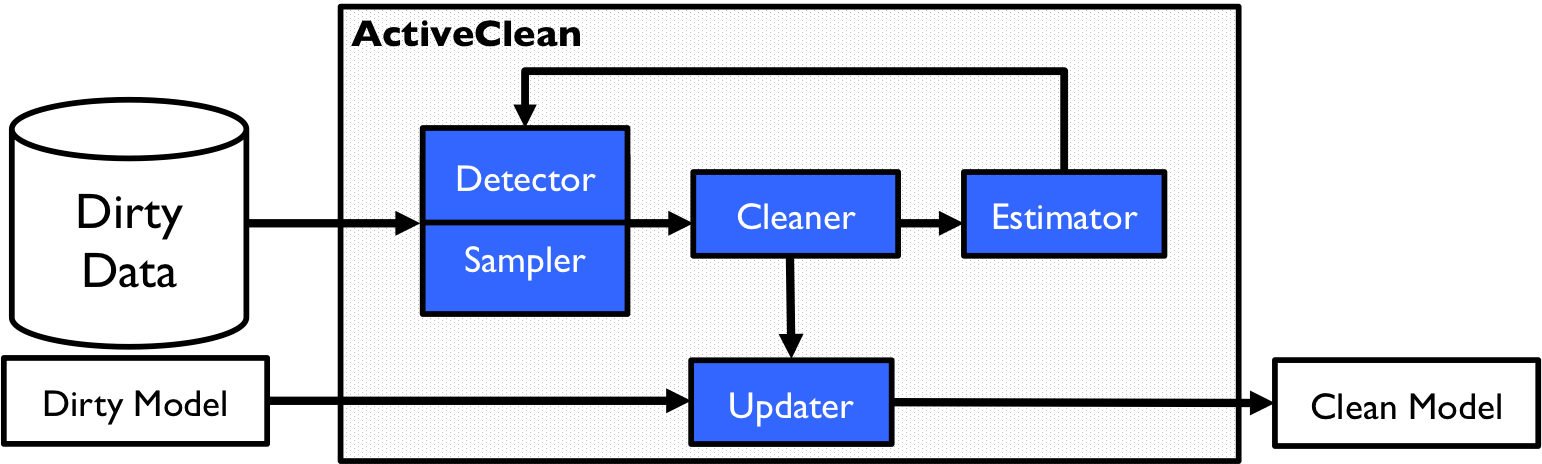
\includegraphics[width=\columnwidth]{figs/arch.png}
 \caption{\sysfull presents an architecture where data cleaning is integrated with model training. The user specifies a data cleaning procedure, and we provide a framework for sampling, model update, and feedback through estimation. \label{sys-arch}}\vspace{-2em}
\end{figure}

In response to these problems, we propose \sys, a framework that integrates existing data cleaning techniques with model training in a way that ensures reliable progressive data cleaning.
Suppose an analyst has a large dirty dataset, a data cleaning technique, a budget of cleaning $k$ records, and a model she wishes to train.
\sys divides the budget into small batches, applies the data cleaning to each batch, and incrementally updates the model after cleaning.
The system is tuned to select the most valuable samples of data to clean based on previous batches of cleaned data. 
\sys can integrate user specified dirty data detection rules (such as constraints) into the framework to further guide our sampling.
The key insight is that the iterative data cleaning and update process can be analyzed as a form of Stochastic Optimization \cite{bertsekas2011incremental} allowing us to leverage convex-analysis theory to develop optimized sampling methods while preserving provable guarantees.

As analytics frameworks increasingly support advanced analytics, tools that encourage reliable methodologies are required.
The incremental updates from \sys give provable bounds on intermediate results, and these results are also viable models that can be used for prediction. 
Specifically, our contributions are:
\begin{itemize}[noitemsep]
\item We propose the \sys framework that tightly integrates data cleaning and model training.
\item (Model Update Section \ref{model-update}) We propose a technique that updates a dirty model from a sample of clean data based on gradient descent. We batch together data that we expect to be clean leading to significant improvements in convergence rate.
\item (Sampling Section \ref{dist-samp}) We derive an optimal sampling distribution, which wcan be approximated by maintaining an estimate of the impact of data cleaning on a record. 
\item (Estimation Section \ref{sampling}) The estimation technique applies linearization to decouple changes in different features allowing us to integrate knowledge about what is wrong with the data (i.e. analyst-specified detection rules) to better estimate error impact.
\item We evaluate \sysfull on real and synthetic datasets to show that our approach gives a sharper cost-accuracy tradeoff than random sampling and Active Learning.
\end{itemize}






